\section{Key exchange process}
\label{chap:key_exchange}


To let all the objects communicate with each other, some public keys must be exchanged during the execution of the POP-C++ application. 
\subsection{Theoretical assumptions}
To be able to implement a version of POP-C++ secured by SSH tunnelling, there are some theoretical assumptions that must be followed.
\begin{enumerate}
\item The main node (the node on which the main program is running) must know all the public keys of every node running a parallel object of the application. This will allow the parallel object to establish a communication with the Application Services running on the main node.
\item The node running a parallel object must know all the public keys of every node which has a reference to this object. This will allow the interface of this parallel object to contact its broker.
\item The node receiving a reference of a parallel object must have the public key of the node who runs this parallel object.
\end{enumerate}




\subsection{Practical point of view}
In a practical point of view, the POP-C++ middle-ware disposes already of some mechanisms that can help the implementation of this security level.\s

\textbf{The access point}\\
The reference of a parallel object is its access point. This access point must hold additional information on the security of the node on which his parallel object is running. The access point must know whether the node must be contacted in a "secure" or "non-secure" way. \\
The access point must also hold the public key of the node on which his parallel object is running.\s

\textbf{The main program}\\
The node A running the main program must know the public key of the node B running a parallel object of this program. This public key must be given in the response of the resource discovery but it should be used only if the parallel object is created on node B.


\pagebreak
\subsection{Scenario}
In this section, there are two scenarios fully explained to understand the whole process of the key exchange in POP-C++. 

\subsubsection{Scenario 1}
In the first scenario illustrated Figure\ref{fig:kex_object_creation} and Figure\ref{fig:kex_ref_passing}, there are 7 nodes running POP-C++. The node "M" is the main node running the "main" of the POP-C++ application.\\
The object creation goes as follow : \s

\begin{enumerate}
\item The main node "M" creates the parallel object "o1" on the node "A" and the parallel object "o4" on the node "D".
\item The object "o1" in Node "A" creates the parallel object "o2" on the Node "B".
\item The object "o2" in Node "B" creates the parallel object "o3" on the Node "C".
\item The object "o4" in Node "D" creates the parallel object "o5" on the Node "E".
\item The object "o5" in Node "E" creates the parallel object "o6" on the node "F".
\end{enumerate}\s

\emph{NOTE:} When an object creates another object, the JobMgr on the node running the object will be contacted.\s

During its creation, a parallel object must give its public key to the main node. After the whole object creation process, the main node will know the public keys of all nodes. \s

When a parallel object is created from another parallel object, the node who creates the object must know the public key of the node who runs the parallel object. This will allow the interface to contact the broker with a secure connection.
\begin{figure}[ht]
	\caption{Scenario 1 : Key exchange during objects creation}
  	\centering
	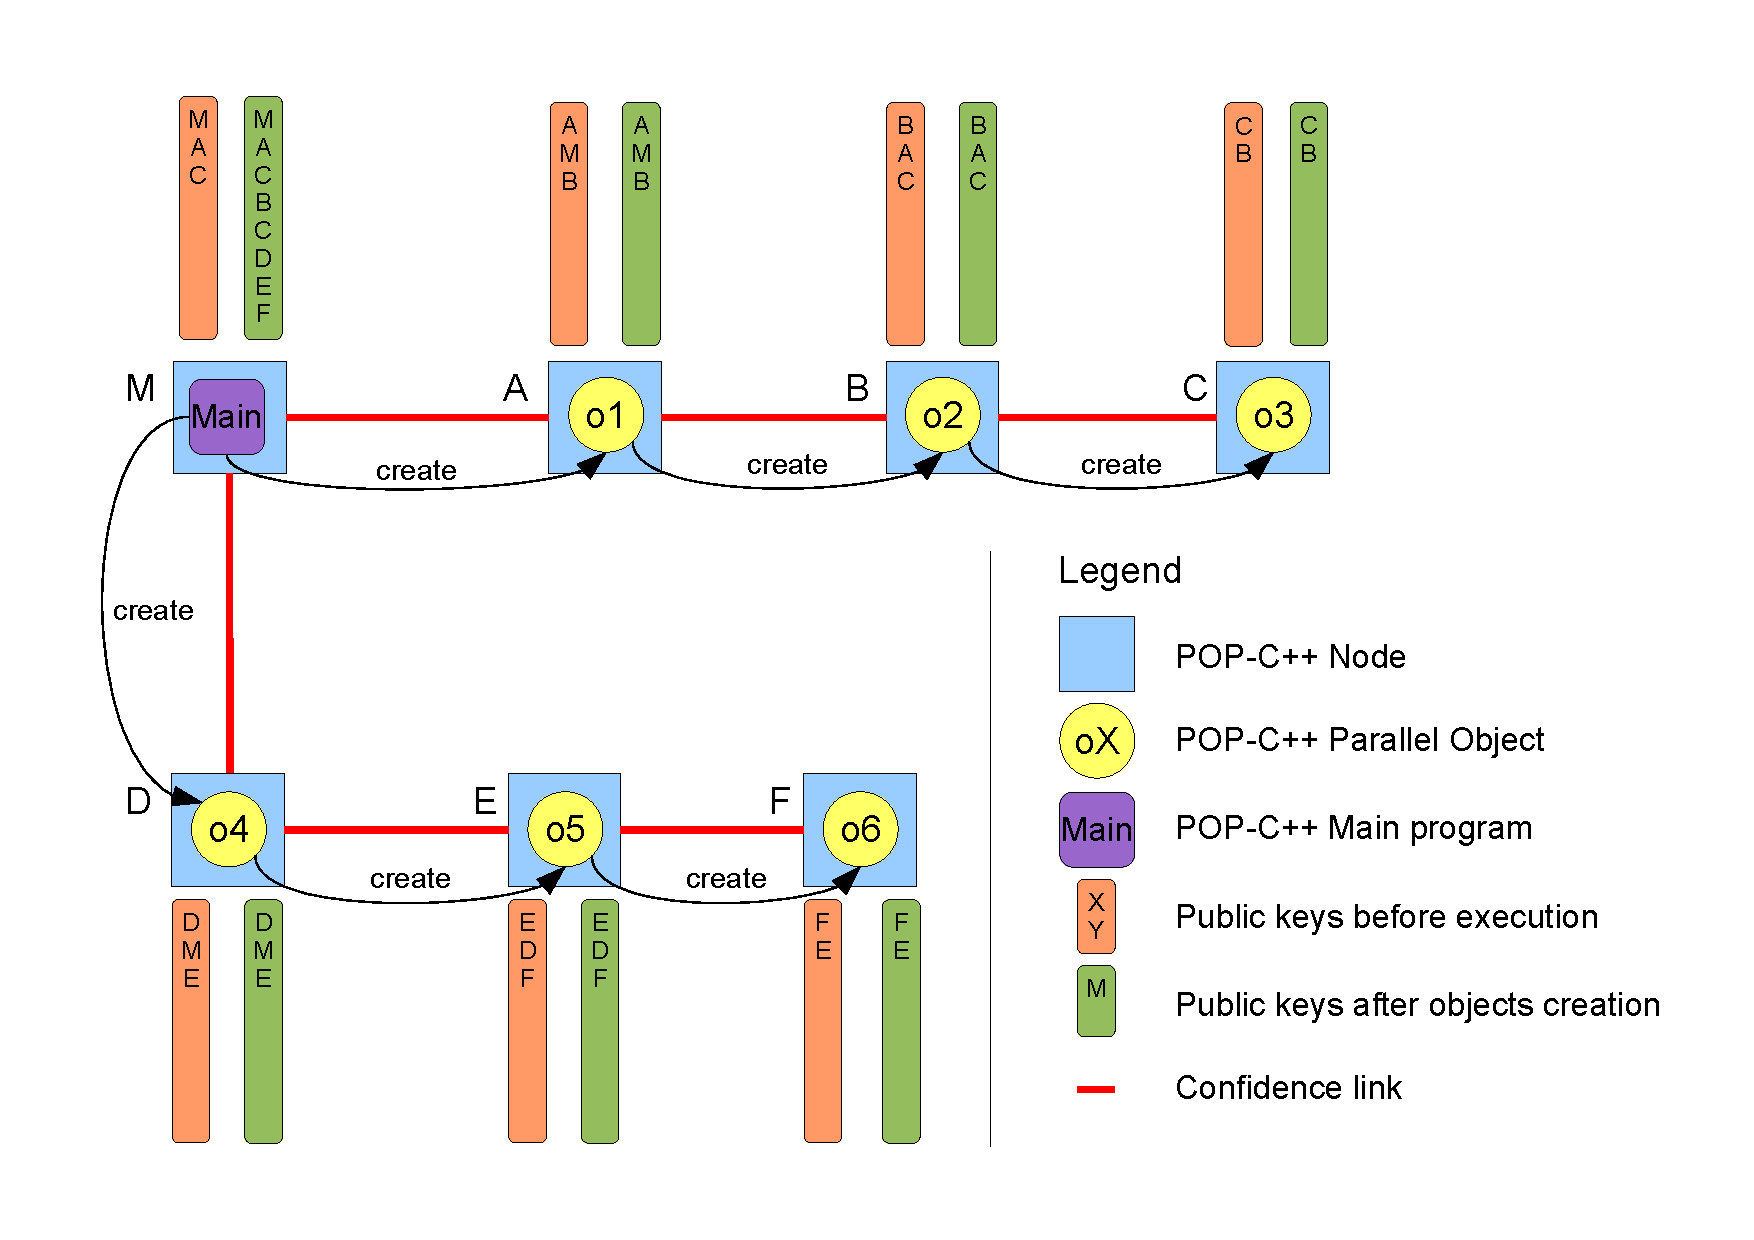
\includegraphics[width=0.7\textwidth]{../object_creation.pdf}
	\label{fig:kex_object_creation}
\end{figure}



\pagebreak


Figure \ref{fig:kex_ref_passing} shows the passing of parallel object reference between parallel objects. This procedure is explained below : 
\begin{enumerate}
\item The node "A" passes the reference of "o2" to the main node. The node running "o2" adds the public key of "M". The node "M" adds the public key of the node running "o2".
\item The node "M" passes the reference of "o2" to the node "D". The node running "o2" adds the public key of "D". The node "D" adds the public key of the node running "o2".
\item The node "D" passes the reference of "o2" to the node "E". The node running "o2" adds the public key of "E". The node "E" adds the public key of the node running "o2".
\item The node "E" passes the reference of "o6" to the node "B". The node running "o6" adds the public key of "B". The node "B" adds the public key of the node running "o6".
\end{enumerate}
\begin{figure}[ht]
	\caption{Scenario 1 : Key exchange during reference passing}
  	\centering
	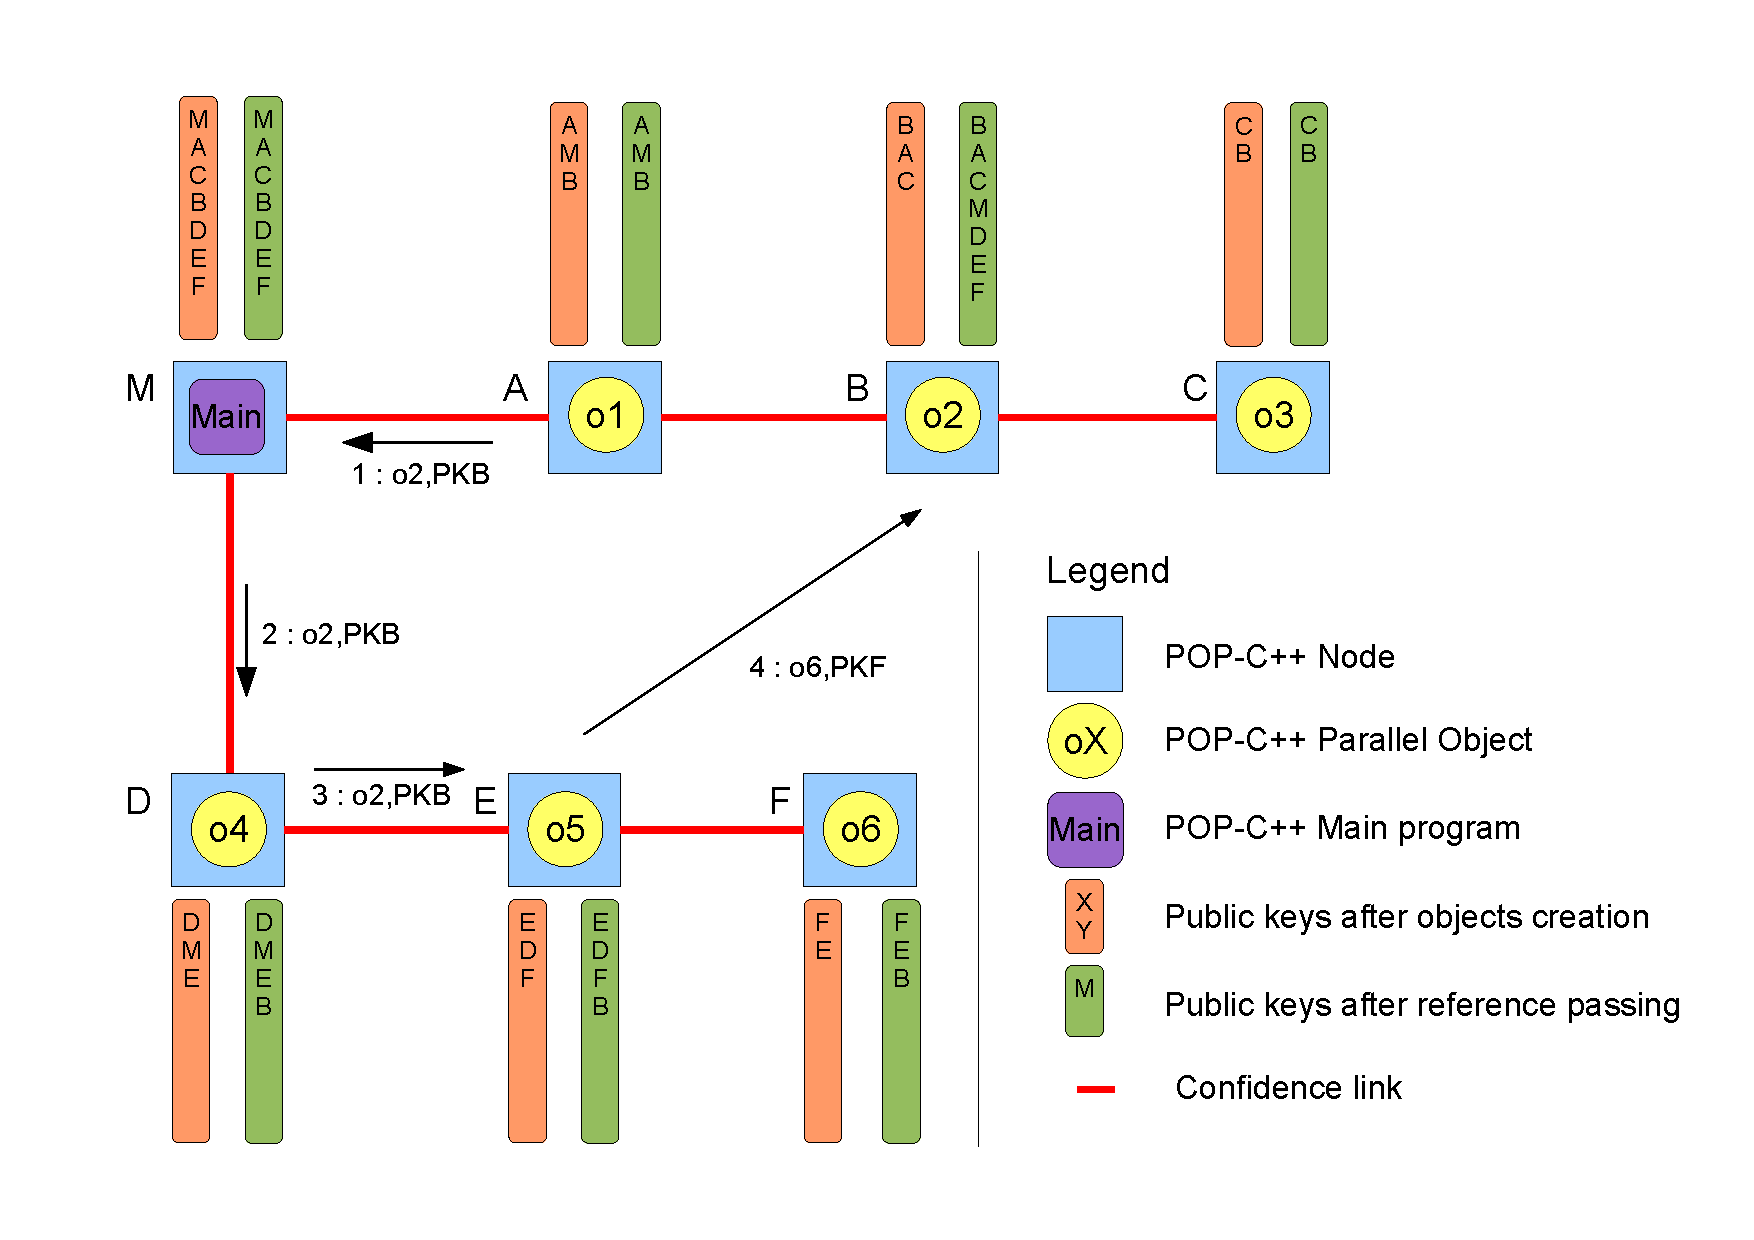
\includegraphics[width=0.8\textwidth]{../ref_passing.pdf}
	\label{fig:kex_ref_passing}
\end{figure}

\pagebreak
\subsubsection{Scenario 2}
In the second scenario, there are 8 nodes running POP-C++. The node running the "main" of the POP-C++ application is the node "C". The objects creation goes as follows : 
\begin{itemize}
\item The node "C" will create the objects "o1", "o5" and "o6". 
\item The node running "o1" will create the objects "o2" and "o4". 
\item The node running "o2" will create the object "o3".
\item The node running "o6" will create the object "o7".
\end{itemize}
Like in the first scenario, the main node will know all the public key. All the parallel objects will be able to communicate with the "Application Services" located on the main node.\\
The node who creates a parallel object gives his public key to the node running this parallel object. This allows the interface to communicate to the broker trough a secure link. 

\begin{figure}[ht]
	\caption{Scenario 2 : Key exchange during objects creation}
  	\centering
	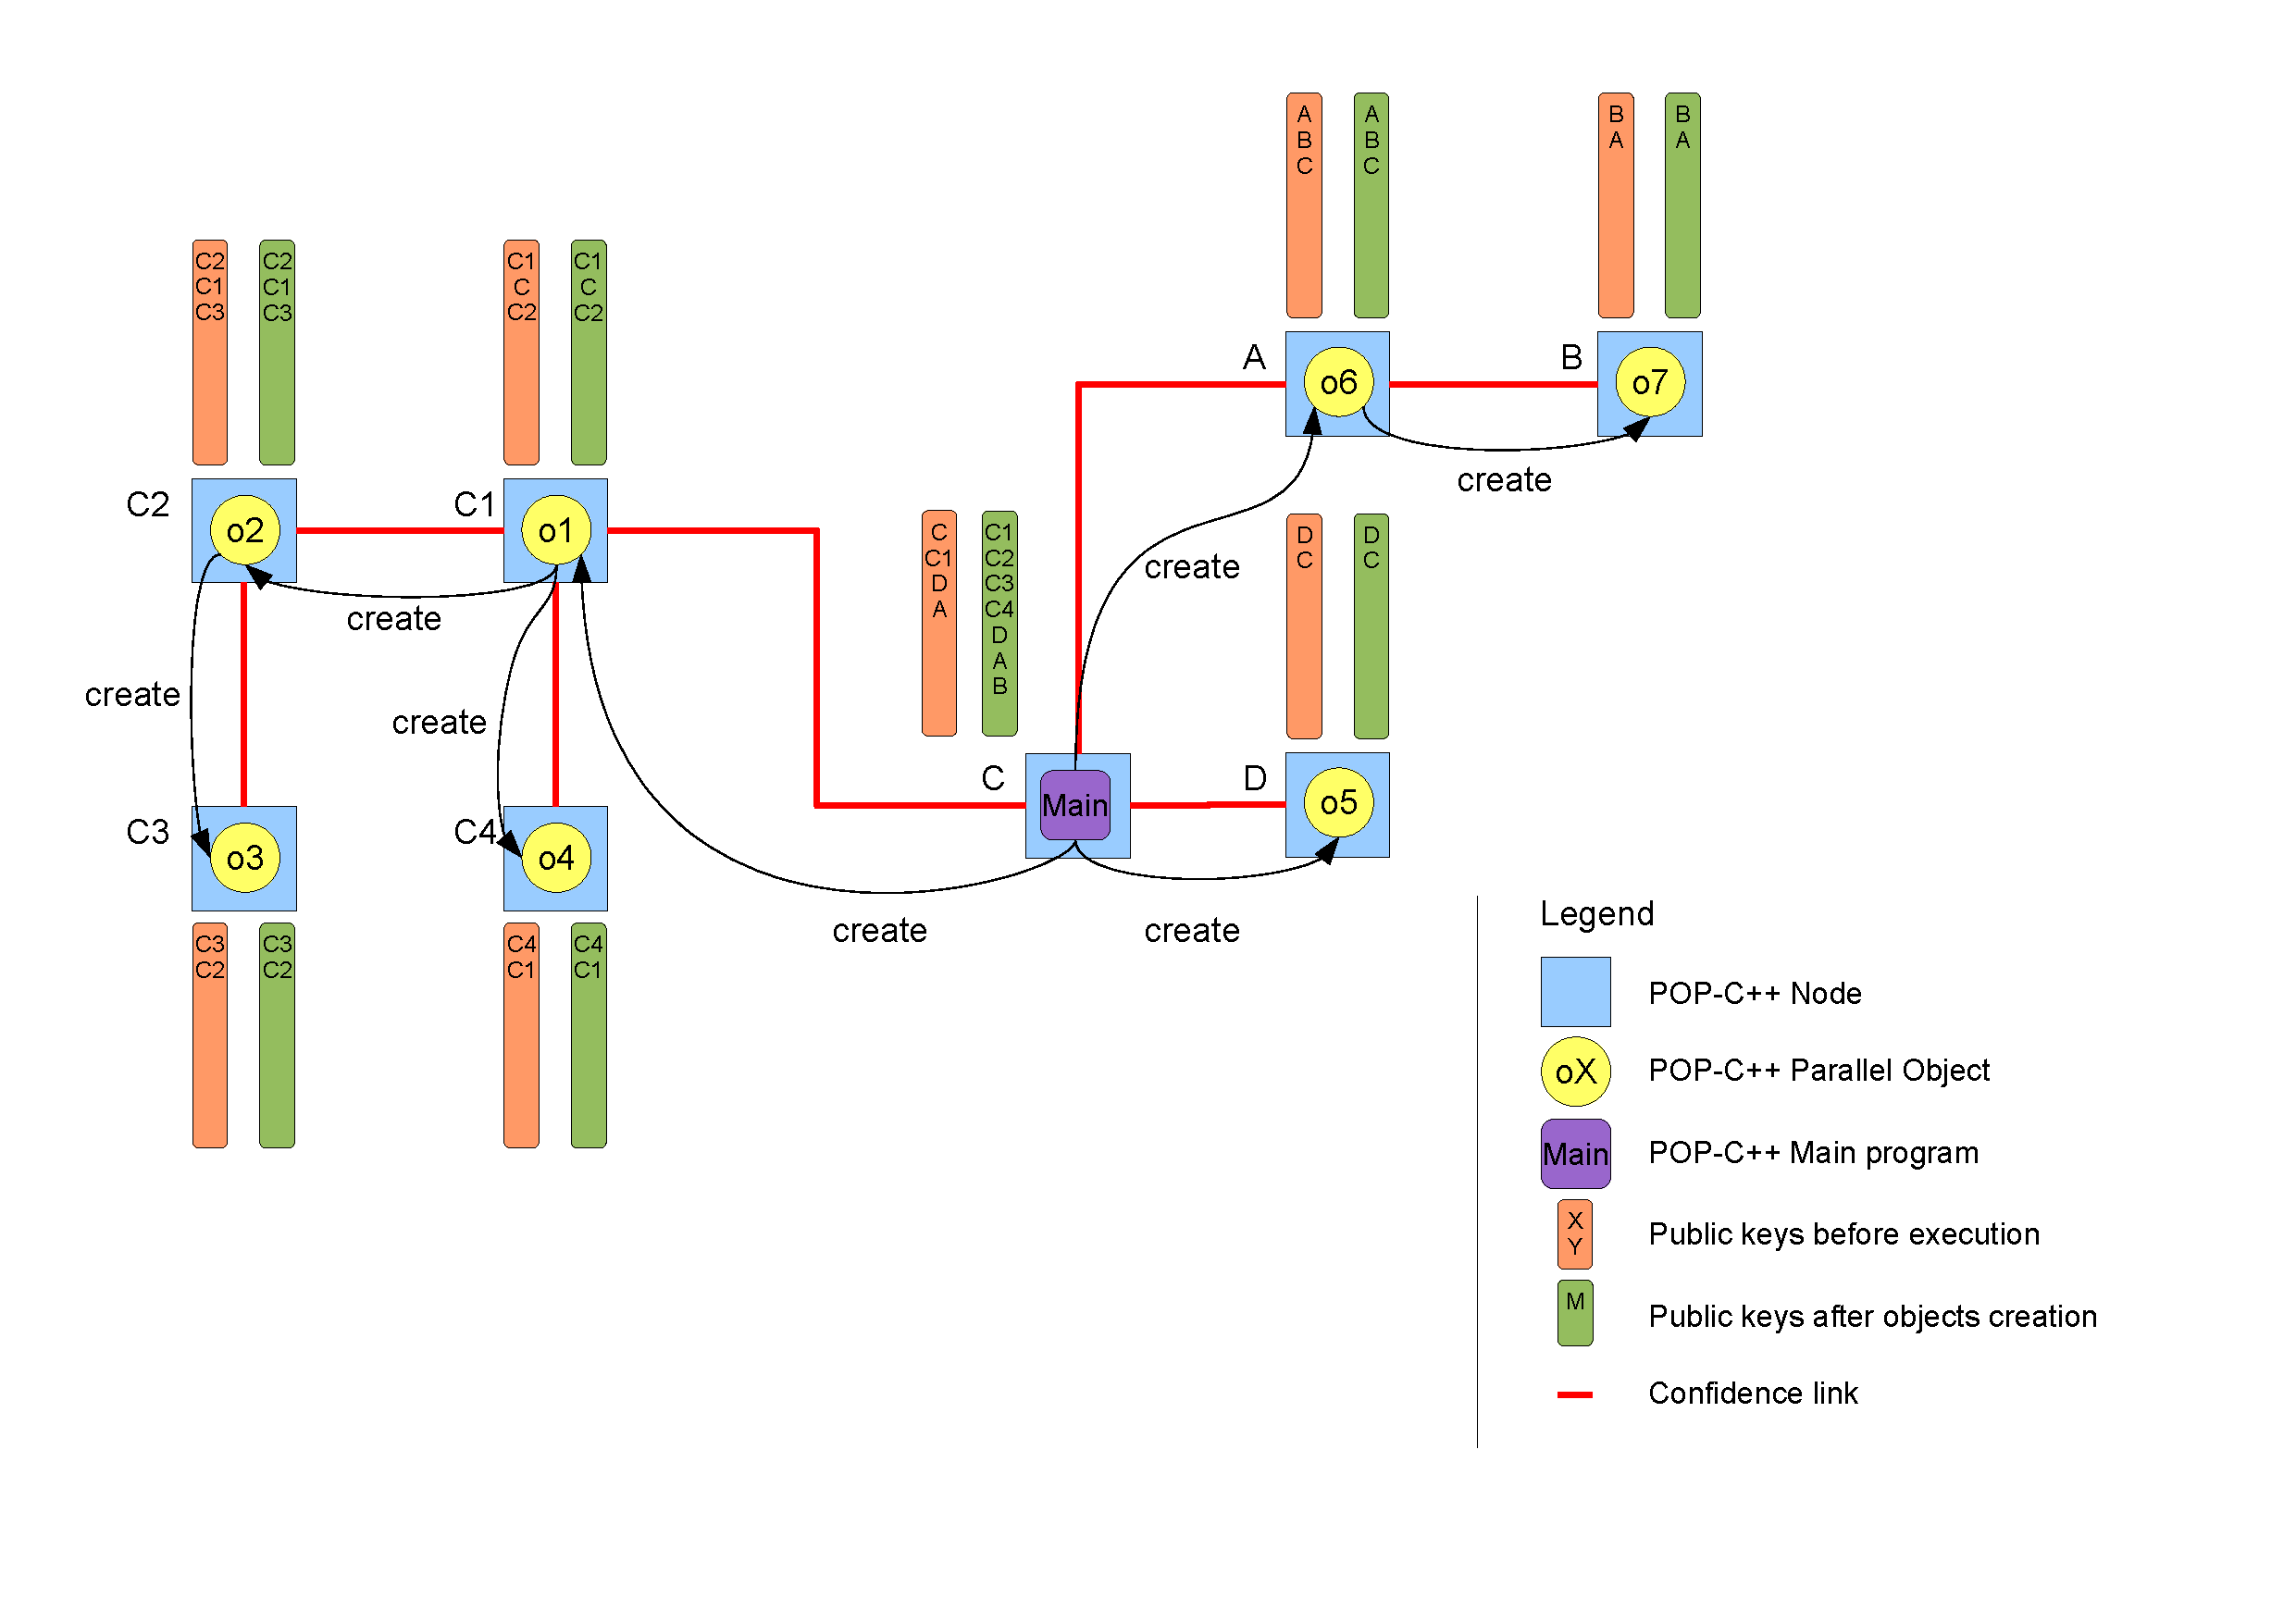
\includegraphics[width=1.0\textwidth]{../sc2-1.pdf}
	\label{fig:kex_object_creation_sc2}
\end{figure}
Once the parallel object creation is done, the program can pass references of parallel object to another parallel object.

\pagebreak

\begin{figure}[ht]
	\caption{Scenario 2 : Key exchange during reference passing}
  	\centering
	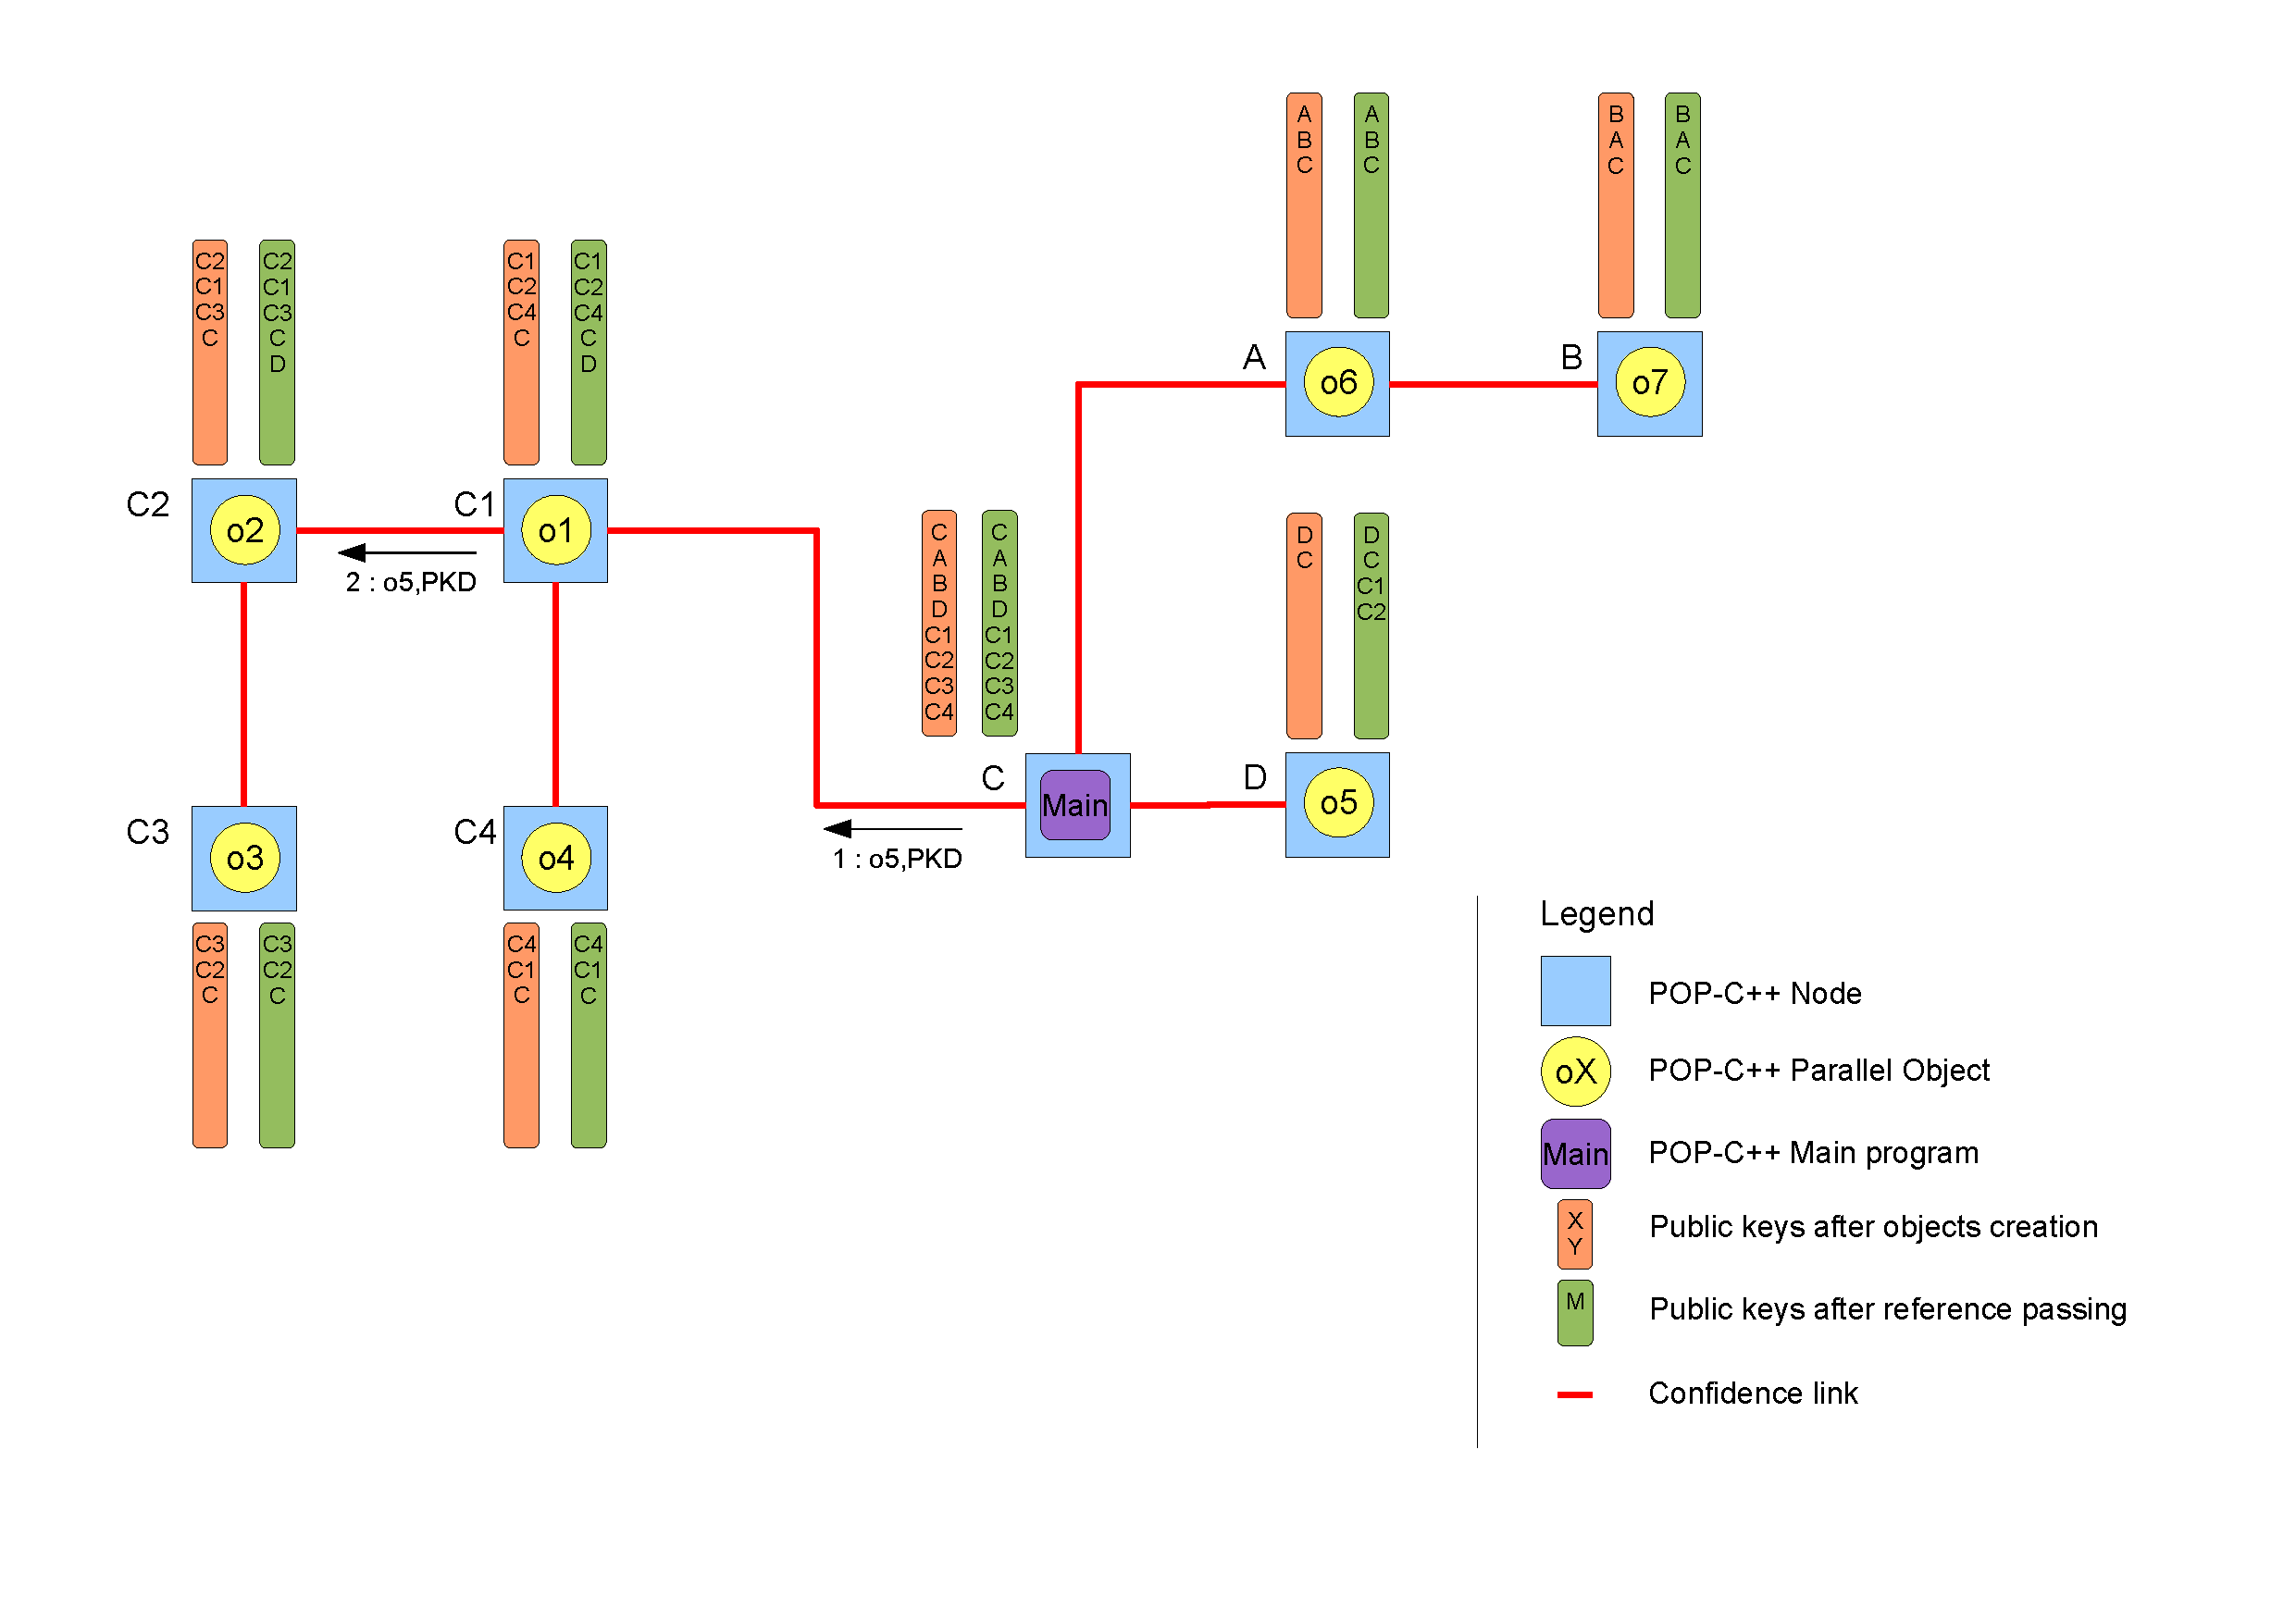
\includegraphics[width=1.0\textwidth]{../sc2-2.pdf}
	\label{fig:kex_ref_passing_sc2}
\end{figure}

In this scenario, the reference of the object "o5" is passed to the node "C1" and after to the node "C2". This reference passing goes like this : \s

\begin{enumerate}
\item The node "C" passes the reference of "o5" to the node "C1". The node running "o5" adds the public key of "C1". The node "C1" adds the public key of the node running "o5".
\item The node "C1" passes the reference of "o5" to the node "C2". The node running "o5" adds the public key of "C2". The node "C2" adds the public key of the node running "o5".
\end{enumerate}\s

The node "C2" is now able to communicate with the parallel object "o5" because the node can create a SSH tunnel between him self and the node "D".